\section{什么是群}\label{sec:1.2}
让我们先从半群讲起.
\begin{Definition}
    集合~$S$~和~$S$~上满足结合律的二元运算~$\cdot$~所形成的代数结构叫做\textbf{半群}.
    这个半群记成~$(S,\cdot)$~或者简记成~$S$,运算~$x \cdot y$~也常常简写成~$xy$~.
\end{Definition}\par
如果运算又满足交换律,则~$(S,\cdot)$~叫做\textbf{交换半群}.象通常那样令
~$x^2=x \cdot x,~x^{n+1}=x^n \cdot x(=x \cdot x^n~,~n \geq 1)$
\begin{Definition}
    设~$S$~是半群,元素~$e \in S$~叫做半群~$S$~的幺元素,是指对每个~$x \in S,~xe=ex=x.$~
\end{Definition}
如果半群~$S$~有幺元素~$e$~,则它是唯一的,因若~$e'$~也是幺元素,则~$e'=e'e=e$~.我们将半群~$S$~中这个
唯一的幺元素(如果存在的话)通常记作~$1_S$~或者~$1$~具有幺元素的半群叫\textbf{含幺半群}.
\begin{Definition}
    设~$S$~是含幺半群.元素~$y \in S$~叫做元素~$x \in S$~的逆元素,是指~$xy=yx=1$.
\end{Definition}
如果~$x$~有逆元素,则它一定唯一.因为若~$y'$~也是~$x$~的逆元素,则~$xy'=y'x=1$.于是
\begin{equation*}
    y=y \cdot 1=y(xy')=(yx)y'=1 \cdot y'=y'.
\end{equation*}
所以若~$x$~具有逆元素,我们把这个唯一的逆元素记作~$x^{-1}$~,则~$xx^{-1}=x^{-1}x=1$~.
\begin{Definition}
    定义半群~$G$~如果有幺元素,并且每个元素均可逆,则~$G$~叫做群.此外,若运算又满足交换律,则~$G$~叫
    做\textbf{交换群}或叫\textbf{阿贝耳(Abel)群}.
\end{Definition}
下面给出半群和群的一些例子.
\begin{example}
    设~$M$~为非负整数全体,~$(M,+)$~是含幺交换半群,幺元素是数~$0$~,但它不是群,因为只有~$0$~对于
    加法在~$M$~中才可逆.
\end{example}\par
$\ZZ,\QQ,\RR,\CC$~对于加法均是阿贝耳群,叫做整数加法群,有理数加法群等等.\par
$(\NN,~\cdot~)$~是含幺交换(乘法)半群,幺元素为~$1$~.它不是群.令~$\QQ\ast$~为非零有理数全体,
则~$(\QQ\ast,~\cdot~)$~是交换群,幺元素为~$1$~,非零有理数~$a$~的乘法逆为~$a^{-1}$~.这叫非零
有理数乘法群,同样有~$(\RR\ast,~\cdot~)$~和~$(\CC\ast,~\cdot~)$~,这些都是阿贝耳群.
\begin{example}
    以~$M_{m,n}(\CC)$~表示全体~$m$~行~$n$~列复矩阵组成的集合,它对矩阵加法形成阿贝耳群.幺元素是全零矩阵,
    而矩阵~$A=(a_{ij})$~的加法逆是~$-A=(-a_{ij})$~.以~$M_n(\CC)$~表示~$n$~阶复方阵全体,它对乘法形成含
    幺半群,幺元素是单位方阵~$I_n$.由线性代数可知,~$n$~阶复方阵~$A$~有乘法逆的充要条件是~$\det A \neq 0$
    .从而~$M_n(\CC)$~不是群,并且当~$n \geq 2$~时,易知半群~$M_n(\CC)$~不是交换的.类似有加法交换群
    ~$M_{m,n}(\RR)$~,含幺半群~$M_{n}(\QQ)$~等等.
\end{example}
\begin{example}
    设~$A$~是非空集合,以~$\sum(A)$~表示从~$A$~到~$A$~全体映射组成的集合.则~$\sum(A)$~对于映射合成运算
    形成含么半群.幺元素为~$A$~上恒等映射~$1_A$~.由1.1的\thmref{yl:1.1.2}可知,~$\sum(A)$~中映射~$f$~
    可逆的充要条件是~$f$~为一一对应.所以当~$|A|>1$~时,~$\sum(A)$~不是群,并且半群~$\sum(A)$~不是交换的.
\end{example}
\begin{example}
    欧氏平面~$\RR^2$~中保持欧氏距离不变的运动叫做\textbf{欧氏运动}.由于欧氏运动必为~$\RR^2$~到自身之上
    的一一对应,并且它的逆仍是欧氏运动,而两个欧氏运动的合成仍是欧氏运动,从而全体欧氏运动形成群,叫做平面
    上的\textbf{欧氏运动群},这也是非阿贝耳群.
\end{example}
\begin{example}
    设~$n$~为正整数,我们在~$\ZZ$~上定义如下关系:对于整数~$a$~和~$b$~,
    \begin{equation*}
        a \sim b \Leftrightarrow n~|~a-b(\mbox{即}~a \equiv b(\mathrm{mod}~n)) 
    \end{equation*}
    易知这是等价关系,于是整数集合~$\ZZ$~分拆成~$n$~个等价类:~$\bar{0},\bar{1},\cdots,\overline{n-1}$~,
    其中~$\bar{i}$~表示~$i$~所在的等价类,即~$\bar{i}=\{m \in \ZZ~|~m \equiv i(\mathrm{mod}~n)\}$~.而
    ~$\{0,1,2,\cdots,n-1\}$~是~$Z$~对于上述模~$m$~同余关系的一个完全代表系.\par
    以~$Z_n$~表示上述~$n$~个等价类组成的集合.在~$Z_n$~上定义加法:
    \begin{equation*}
        \bar{a}+\bar{b}=\overline{a+b}
    \end{equation*}
    由同余式基本性质可知这个加法运算是可以定义的,即与等价类(或叫\textbf{模~$n$~同余类})中代表元的取法无关
    ,并且~$Z_n$~对于这个运算形成交换群,幺元素是~$\bar{0}$,这叫\textbf{整数模~$n$~加法群}.\par
    如果~$Z_n$~中定义乘法
    \begin{equation*}
        \overline{a}\overline{b}=\overline{ab}
    \end{equation*}
    则~$Z_n$~对此乘法是含么交换半群,幺元素为~$\bar{1}$~.由于等式~$\bar{a}\bar{b}=\bar{1}$~相当于同余式
    ~$ab \equiv 1(\mathrm{mod}~n)$~.从初等数论知道,对于给定的~$a$~,存在~$b$~满足
    ~$ab \equiv 1(\mathrm{mod}~n)$~的充要条件是~$(a,n)=1$.从而~$a$~对于上述乘法可逆的充要条件是
    ~$(a,n)=1$.
\end{example}
设~$(M,~\cdot~)$~是含幺半群,我们以~$U(M)$~或者~$M*$~表示半群~$M$~中可逆元素全体.
\begin{Definition}
    若~$(M,~\cdot~)$~是含幺半群,则~$(U(M),~\cdot~)$~是群.
\end{Definition}
\begin{proof}
    由~$1_M^{-1}=1_{M}$~可知~$1=1_M \in U(M)$~.若~$a,b \in U(M)$~,则~$a,b$~均可逆,易知~$b^{-1}a^{-1}$~
    是~$ab$~的逆元素,从而~$ab \in U(M)$~.因此~$\cdot$~是~$U(M)$~上的二元运算.这运算在~$U(M)$~中当然
    也满足结合律,于是~$(U(M),~\cdot~)$~是含幺半群.由于~$U(M)$~中每个元素~$a$~均可逆,从而~$a^{-1} \in M$~
    也可逆(因为~$a$~是~$a^{-1}$~的逆),因此~$a^{-1} \in U(M)$~.从而~$U(M)$~中每个元素在~$U(M)$~中均
    可逆.根据定义,~$U(M)$~为群.
\end{proof}
于是由前面的例子便知:\par
\begin{enumerate}
    \item 全体~$n$~阶可逆复方阵形成乘法群,叫做复数上的~$n$~次\textbf{一般线性群},表示成~$GL(n,\CC)$~.同样有群~$GL(n,\RR)$,\par
    $GL(n,\QQ)$~等.
    \item 设~$A$~为非空集合,~$A$~到自身之上的所有一一对应对于合成运算形成群,叫做集合~$A$~上的\textbf{对称群}或\textbf{全置换群},表示成~$S(A)$~,其中元素(即~$A$~到~$A$~的一一对应)叫做集合~$A$~上的\textbf{置换}.
    \item 设~$n$~为正整数,~$\bar{a}$~为整数~$a$~的模~$n$~同余类.则集合则集合
    \begin{equation*}
        Z^*_n = \{\bar{a}~|~(a,n)=1\}
    \end{equation*}
\end{enumerate}
对于乘法形成阿贝耳群.这个群有~$\varphi(n)$~个元素,其中~$\varphi(n)$~是~$1$~到~$n$~中与~$n$~互素的整数个数($\varphi(n)$~叫\textbf{欧拉函数}).\par
设~$G$~是群.若集合~$G$~有限,称~$G$~为有限群,否则叫无限群.若有限群~$G$~共有~$n$~个元素,则~$G$~叫~$n$~\textbf{阶群}或叫~$n$~\textbf{元群},~$n=|G|$~叫有限群~$G$~的\textbf{阶}.\par
为了考查各种群之间的联系,我们要研究群之间的映射.但是群不仅是集合还有运算,所以我们需要映射与群运算保持协调.确切地说:
\begin{Definition}
    设~$(G,\cdot)$~和~$(G',\circ)$~是两个群.映射~$f:G \to G'$~叫做群~$G$~到群~$G'$~的同态,是指对~$a,b\in G$~
\end{Definition}
$f(a \cdot b) = f(a) \circ f(b)$(简记为~$f(ab)=f(a)f(b)$).
此外,若~$f$~又为单射或满射,则~$f$~分别叫\textbf{单同态}或\textbf{满同态}.如果同态~$f$~是一一对应,则称~$f$~是群~$G$~到群~$G'$~的同构.这时,称群~$G$~和~$G'$~是同构的,表示成~$G=G'$~或者~$f:G\underrightarrow{\sim}G'$~.

\newpage
\begin{figure}[htbp]
    \centering
    \includegraphics[scale=0.6]{Figure/old/2.pdf}
    \caption{}\label{fig:2}
\end{figure}

\begin{figure}[htb]
    \centering
    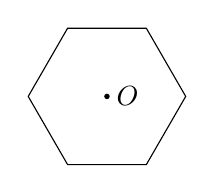
\begin{tikzpicture}
        \draw (0,0) -- (0.5,0.866) -- (1.5,0.866) -- (2,0)
         -- (1.5,-0.866) -- (0.5,-0.866) -- cycle;
        \fill (1,0) circle[radius=1pt] node[right] {$O$};
    \end{tikzpicture}
    \caption{正六边形}
\end{figure}
